\documentclass{amsart}

\linespread{2}
% \usepackage{fontspec}
% \setmainfont{Open Dyslexic}


% PACKAGES ~~~~~~~~~~~~~~~~~~~~

\usepackage{amsfonts}
\usepackage{amssymb}  
\usepackage{amsthm} 
\usepackage{amsmath} 
\usepackage{caption}
\usepackage[inline]{enumitem}
\setlist{itemsep=0em, topsep=0em, parsep=0em}
\setlist[enumerate]{label=(\alph*)}
\usepackage{etoolbox}
\usepackage{stmaryrd} 
\usepackage[dvipsnames]{xcolor}
\definecolor{editcolour}{rgb}{0.7,0.1,0}
\definecolor{hrefcolour}{rgb}{0,0,0.7}

\usepackage[]{hyperref}
\hypersetup{colorlinks,linkcolor={hrefcolour},citecolor={hrefcolour},urlcolor={hrefcolour}}
\usepackage{graphicx}
\graphicspath{ {img/} }
\usepackage{mathtools}

\usepackage{tikz}
\usetikzlibrary{matrix,arrows,shapes,decorations.markings,decorations.pathreplacing}
\usepackage{todonotes}

% NEW COMMANDS ~~~~~~~~~~~~~~~~~~

% symbols
\renewcommand{\epsilon}{\varepsilon}
\newcommand{\op}{^{\scriptsize{ \textrm{op} } }}
\newcommand{\iso}{\cong}
\renewcommand{\equiv}{\simeq}

% categories
\newcommand{\A}{\cat{A}}
\newcommand{\B}{\cat{B}}
\newcommand{\C}{\cat{C}}
\newcommand{\D}{\cat{D}}
\newcommand{\E}{\cat{E}}
\renewcommand{\P}{\cat{P}}
\newcommand{\Q}{\cat{Q}}
\newcommand{\R}{\cat{R}}
\newcommand{\T}{\cat{T}}
\newcommand{\U}{\cat{U}}
\newcommand{\V}{\cat{V}}
\newcommand{\W}{\cat{W}}
\newcommand{\X}{\cat{X}}
\newcommand{\Y}{\cat{Y}}
\newcommand{\Z}{\cat{Z}}
\renewcommand{\AA}{\bicat{A}}
\newcommand{\BB}{\bicat{B}}
\newcommand{\CC}{\bicat{C}}
\newcommand{\DD}{\bicat{D}}
\newcommand{\EE}{\bicat{E}}
\newcommand{\PP}{\bicat{P}}
\newcommand{\QQ}{\bicat{Q}}
\newcommand{\RR}{\bicat{R}}
\newcommand{\TT}{\bicat{T}}
\newcommand{\UU}{\bicat{U}}
\newcommand{\VV}{\bicat{V}}
\newcommand{\WW}{\bicat{W}}
\newcommand{\XX}{\bicat{X}}
\newcommand{\YY}{\bicat{Y}}
\newcommand{\ZZ}{\bicat{Z}}
\newcommand{\AAA}{\dblcat{A}}
\newcommand{\BBB}{\dblcat{B}}
\newcommand{\CCC}{\dblcat{C}}
\newcommand{\DDD}{\dblcat{D}}
\newcommand{\EEE}{\dblcat{E}}
\newcommand{\MMM}{\dblecat{M}}
\newcommand{\PPP}{\dblcat{P}}
\newcommand{\QQQ}{\dblcat{Q}}
\newcommand{\RRR}{\dblcat{R}}
\newcommand{\SSS}{\dblcat{S}}
\newcommand{\TTT}{\dblcat{T}}
\newcommand{\UUU}{\dblcat{U}}
\newcommand{\VVV}{\dblcat{V}}
\newcommand{\WWW}{\dblcat{W}}
\newcommand{\XXX}{\dblcat{X}}
\newcommand{\YYY}{\dblcat{Y}}
\newcommand{\ZZZ}{\dblcat{Z}}

\newcommand{\Set}{\cat{Set}}
\newcommand{\Rel}{\cat{Rel}}
\newcommand{\Pos}{\cat{Pos}}
\newcommand{\Graph}{\cat{Graph}}
\newcommand{\RGraph}{\cat{RGraph}}
\newcommand{\Top}{\cat{Top}}
\newcommand{\Cat}{\cat{Cat}}
\newcommand{\Bicat}{\cat{Bicat}}
\newcommand{\DblCat}{\cat{DblCat}}
\newcommand{\Topos}{\cat{Topos}}
\newcommand{\Span}{\cat{Span}}
\newcommand{\Csp}{\cat{Cospan}}
\newcommand{\Gram}{\cat{Gram}}
\newcommand{\StrCsp}{\cat{StrCsp}}
\newcommand{\SSStrCsp}{\dblcat{S} \cat{trCsp}}
\newcommand{\StrCspGram}{\cat{StrCspGram}}
\newcommand{\MonSpCsp}{\dblcat{M} \cat{onSpCsp}}

% functors
\newcommand{\core}{\mathbf{core}}
\newcommand{\Lang}{\mathrm{Lang}}

% text formatting
\newcommand{\defn}[1]{\textbf{#1}}
\newcommand{\cat}[1]{\mathsf{#1}}
\newcommand{\bicat}[1]{\mathbf{#1}}
\newcommand{\dblcat}[1]{\mathbb{#1}}
\newcommand{\type}[1]{\mathtt{#1}}
\newcommand{\edit}[1]{\textcolor{editcolour}{(#1)}}

% arrows
\newcommand{\from}{\colon}
\newcommand{\rel}{\nrightarrow}
\newcommand{\To}{\Rightarrow}
\newcommand{\xto}[1]{\xrightarrow{#1}}
\newcommand{\monicto}{\rightarrowtail}
\newcommand{\dderiv}[2]{#1 \rightsquigarrow #2}
\newcommand{\deriv}[2]{#1 \rightsquigarrow^\ast #2}
\renewcommand{\gets}{\leftarrow}
\newcommand{\monicgets}{\leftarrowtail}
\newcommand{\xgets}[1]{\xleftarrow{#1}}
\newcommand{\spn}[3]{#2 \to #1 \times #3}
\newcommand{\tospan}{\xrightarrow{\mathit{sp}}}
\newcommand{\csp}[3]{#1 + #3 \to #2}
\newcommand{\tocospan}{\xrightarrow{\mathit{csp}}}

% OPERATORS ~~~~~~~~~~~~~~~~~~

\DeclareMathOperator{\Hom}{Hom}
\DeclareMathOperator{\id}{id}
\DeclareMathOperator{\im}{im}
\DeclareMathOperator{\Sub}{Sub}
\DeclareMathOperator{\colim}{colim}

% ENVIRONMENTS & COUNTERS ~~~~~~~~~~~

\newtheorem{theorem}{Theorem}[section]
\newtheorem{lemma}[theorem]{Lemma}
\newtheorem{proposition}[theorem]{Proposition}
\newtheorem{corollary}[theorem]{Corollary}

\theoremstyle{remark}
\newtheorem{remark}[theorem]{Remark}
\newtheorem{notation}[theorem]{Notation}

\theoremstyle{definition}
\newtheorem{example}[theorem]{Example} 
\newtheorem{definition}[theorem]{Definition}

\setcounter{tocdepth}{1} % Sets depth for table of contents. 

% TIKZ TYPES ~~~~~~~~~~~~~~~~~~~~~

% arrow head in middle of edge
\tikzset{->-/.style={decoration={%
      markings,
      mark=at position .5 with {\arrow{>}}},postaction={decorate}}
}

% arrow head user-positioned
\tikzset{->-pos/.style={decoration={%
      markings,
      mark=at position #1 with {\arrow{>}}},postaction={decorate}}
}

% arrow head in middle of edge
\tikzset{-|->/.style={decoration={%
      markings,
      mark=at position .5 with {\arrow{|}},mark=at position 1 with {\arrow{>}}},postaction={decorate}}
}

% INLINE DIAGRAMS ~~~~~~~~~~~~~~~

% walking reflexive graph
\newcommand{\rgraph}[2]{%
  \begin{tikzpicture}[scale=0.75,baseline=-3pt]
    \node (a) at (0,0) {$ #1 $};
    \node (b) at (1,0) {$ #2 $};
    \draw [->]
    ([yshift= 4pt]a.east) to ([yshift= 4pt]b.west);
    \draw [->]
    ([yshift=-4pt]a.east) to ([yshift=-4pt]b.west);
    \draw [->]
    (b.west) to (a.east);
  \end{tikzpicture}
}

% walking graph
\newcommand{\graph}[2]{%
  \begin{tikzpicture}[scale=0.75,baseline=-3pt]
    \node (a) at (0,0) {$ #1 $};
    \node (b) at (1,0) {$ #2 $};
    \draw [->]
    ([yshift=4pt]a.east) to ([yshift=4pt]b.west);
    \draw [->]
    ([yshift=-4pt]a.east) to ([yshift=-4pt]b.west);
  \end{tikzpicture}
}

% open tipped arrow
\newcommand{\opento}[2]{%
  \begin{tikzpicture}[scale=0.75,baseline=-3pt]
    \node (a) at (0,0) {$ #1 $};
    \node (b) at (1,0) {$ #2 $};
    \draw [->, open triangle 60]
    (a.east) to (b.west);
  \end{tikzpicture}
}

% inline horizontal arrow
\newlength\mylen
\settowidth\mylen{$\to$}

\newcommand{\horarrow}{%
  \to\kern-0.55\mylen\vline height 1.2ex depth
  -0.4pt\kern0.55\mylen}

% adjunction
\newcommand{\adjunction}[4]{%
  \begin{tikzpicture}[baseline=-3pt]
    \node (1) at (0,0) {\( #1 \)};
    \node (2) at (2,0) {\( #4 \)};
    \draw [->]
    ([yshift= 4pt]2.west) to
    node [above] {\scriptsize{ $ #2 $ }}
    ([yshift= 4pt]1.east);
    \draw [->]
    ([yshift= -4pt]1.east) to
    node [below] {\scriptsize{ $ #3 $ }}
    node [above,yshift= -1.5pt] {\scriptsize{$ \perp $}}
    ([yshift= -4pt]2.west);
  \end{tikzpicture}
  % 
}

% ~~~~~~~~~~~~~~~~~~~~~~~~~~~~~~~~~~~~~~~~
% 
% ~~~~~~~~~~~ begin document~~~~~~~~~~~~~~
% 
% ~~~~~~~~~~~~~~~~~~~~~~~~~~~~~~~~~~~~~~~~

\begin{document}

This paper fits into a program interested in categorifying the study
of compositional systems.  Part of the motivation for this program is
the desire to understand global behavior of systems through analyzing
local components.  To this end, we are introducing a sytactical
device, structured cospans, to reason about open systems.

In the study of formal languages, often accompanying a syntax is a
rewriting system.  This is a set of rules dictating when one may
replace one syntactical term for another.  Each rewriting system gives
rise to a rewriting relation, which is useful in situations where
distinct syntactical terms have the same semantics, or meaning.  An
example of this arises in electrical circuits when a pair of
resistors are wired in series. This has the same behavior as a single
resistor whose resistance is the sum of the two original resistors.
Syntacitally, these are different components, but we want to treat
them the same.  So an appropriate rewriting system would want to
relate (not equate) these two circuits.   In this paper, we introduce
the theory of rewriting structured cospans.

The theory of rewriting has gone through several epochs, each more
abstract from the last.  Rewriting was introduced by Chomsky for
formal languages. Here, the syntactical terms in consideration were
strings of characters, or letters.  Later, Ehrig,
et.~al. \cite{graphtrans} used pushouts to introduce rewriting for
graphs.  Graph rewriting was then axiomatised by Lack and
Soboci\'{n}ski when they defined adhesive categories
\cite{LackSobo_Adhesive}.  While we do not need the full generality of
adhesive categories, we do use rewriting of topoi, which are examples
of adhesive categries \cite{LackSobo_ToposIsAdh}.

We define a \emph{grammar} to be a topos $ \X $ paired with a
set of rules $ P $.  Each rule in $ P $ is a span
$ \ell \monicgets k \monic r $ in $ \X $ such that each leg is monic.
The conceipt is that the object $ \ell $ can be replaced by $ r $
while the common subobject $ k $ is fixed.  The grammar $ ( \X , P ) $
induces a \emph{derived grammar} $ ( \X , P' ) $ where $ P' $ is
comprised of any rules appearing on the bottom row of a double pushout
diagram of form
%
\[
  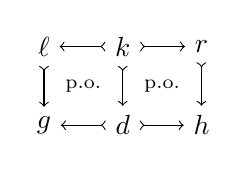
\begin{tikzpicture}
    \node (1) at (0,1) {$ \ell $};
    \node (2) at (1,1) {$ k $};
    \node (3) at (2,1) {$ r $};
    \node (4) at (0,0) {$ g $};
    \node (5) at (1,0) {$ d $};
    \node (6) at (2,0) {$ h $};
    \draw [>->] (2) to node [] {\scriptsize{$  $}} (1);
    \draw [>->] (2) to node [] {\scriptsize{$  $}} (3);
    \draw [>->] (5) to node [] {\scriptsize{$  $}} (4);
    \draw [>->] (5) to node [] {\scriptsize{$  $}} (6);
    \draw [>->] (1) to node [] {\scriptsize{$  $}} (4);
    \draw [>->] (2) to node [] {\scriptsize{$  $}} (5);
    \draw [>->] (3) to node [] {\scriptsize{$  $}} (6);
    \node () at (0.5,0.5) {\scriptsize{p.o.}};
    \node () at (1.5,0.5) {\scriptsize{p.o.}};
  \end{tikzpicture}
\]
%
whose top row belongs to $ P $. The study of the grammar
$ ( \X , P ) $ is really done by understanding the \emph{rewrite
  relation} $ \deriv{g}{h} $ defined by, first, relating objects if
there is a rule in $ P' $ between them, then taking the reflexive and
transitive closure.

In practice, we take $ \X $ to be a topos which we consider to be
comprised of systems together with the appropriate morphisms.  Because
of the important status that graphs play in the field of network
theory, the archetypal topos for us is the category $ \RGraph $ of
reflexive graphs.  Given a rewriting system $ ( \X , P ) $, our goal
is to see how we can rewrite systems $ x $ by somehow decomposing it
into subsystems, rewriting those, then glueing the results back
together.  We claim that, using structured cospans, we can do this in
a way that characterizes the rerwriting relation for $ ( \X , P ) $.

To accomplish this, we turn to Gadducci and Heckle
\cite{Gadd_IndGraphTrans} who introduced an inductive perspective for
graph rewriting.  This is closely related to our present goals so,
while we work in a more general context and have different
motivations than they do, we follow the framework set in their
paper.  In particular, they define so called ``ranked graphs'' which
are directed graphs with a chosen set of nodes serving as inputs and
outputs.  Using structured cospans, we are able to provide inputs and
outputs to a much wider class of objects than graphs. 

To do so, we need addition data besides just $ \X $.  We begin with a
geometric morphism
%
\[
  ( L \from \A \to \X ) \dashv ( R \from \X \to \A ),
\]
% 
which, recall, is an adjunction between topoi whose left adjoint preserves finite
limits.  In this setup, $ \X $ still is our topos of systems.  The new
data consists of $ \A $ which is a topos comprised of ``interface
types''.  These will serve as the boundaries along which we decompose
the systems in $ \X $.  The left adjoint $ L $ serves as the channel
through which we port the interface types into $ \X $ so that they can
interact with the systems.  The fact that this data comes in the form
of a geometric morphism is used throughout this paper.

A \emph{structured cospan} is a cospan in $ \X $ of the form
$ La \to x \gets Lb $. This should be thought of as consisting of a
system $ x $ with inputs $ a $ and outputs $ b $.

Structured cospans were introduced by Baez and Courser
\cite{courser-strcsp}, though under weaker hypothesis than we have here.
We ask for stronger assumptions in order to introduce rewriting, which
they do not consider.  Their primary focus was on the compositional
structure, which is captured as follows. A structured cospan
$ La \to x \gets Lb $ with outputs $ b $ can be connected together
with a structured cospan $ Lb \to y \gets Lc $ with inputs $ b $ via
pushout
%
\[
  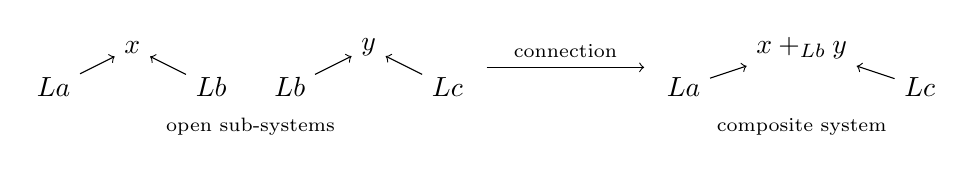
\begin{tikzpicture}
    \begin{scope}
      \node (1) at (0,0) {$ La $};
      \node (2) at (1,0.5) {$ x $};
      \node (3) at (2,0) {$ Lb $};
      \node (4) at (3,0) {$ Lb $};
      \node (5) at (4,0.5) {$ y $};
      \node (6) at (5,0) {$ Lc $};
      \draw [->] (1) to node [] {\scriptsize{$  $}} (2);
      \draw [->] (3) to node [] {\scriptsize{$  $}} (2);
      \draw [->] (4) to node [] {\scriptsize{$  $}} (5);
      \draw [->] (6) to node [] {\scriptsize{$  $}} (5);
      \node () at (2.5,-0.5) {\scriptsize{open sub-systems}};
    \end{scope}
    %
    \begin{scope}[shift={(8,0)}]
      \node (1) at (0,0) {$ La $};
      \node (2) at (1.5,0.5) {$ x +_{Lb} y $};
      \node (3) at (3,0) {$ Lc $};
      \draw [->] (1) to node [] {\scriptsize{$  $}} (2);
      \draw [->] (3) to node [] {\scriptsize{$  $}} (2);
      \node () at (1.5,-0.5) {\scriptsize{composite system}};
    \end{scope}
    %
    \draw [->] (5.5,0.25) to node [above] {\scriptsize{connection}} (7.5,0.25);    
  \end{tikzpicture}
\]
% 
This gives us a category $ \Csp_L $ whose objects are from $ \A $ and
whose arrows are the structured cospans. 

Observe that a system $ x $ without inputs and outputs can be encoded
using the structured cospan $ L0 \to x \gets L0 $.  Studying $ x $
locally means finding a decomposition
%
\[
  L0 \to x_1 \gets Lb_1 \to x_2 \gets Lb_2 \dotsm Lb_{n-1} \to x_n
  \gets L0
\]
% 
and individually looking at each factor. This is exactly what we
intend to do with rewriting.  

To do so, we need to put forward another perspective of structured
cospans.  Namely, we view them as objects with arrows of their own.
These arrows are commuting diagrams
%
\begin{equation} \label{eq:StrCsp-arrows}
\raisebox{-4.5ex}{
  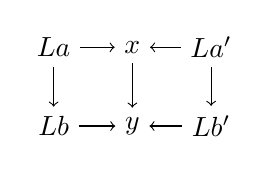
\begin{tikzpicture}
    \node (1t) at (0,1) {$ La $};
    \node (2t) at (1,1) {$ x $};
    \node (3t) at (2,1) {$ La' $};
    \node (1b) at (0,0) {$ Lb $};
    \node (2b) at (1,0) {$ y $};
    \node (3b) at (2,0) {$ Lb' $};
    \draw [->] (1t) to node [] {\scriptsize{$  $}} (2t);
    \draw [->] (3t) to node [] {\scriptsize{$  $}} (2t);
    \draw [->] (1b) to node [] {\scriptsize{$  $}} (2b);
    \draw [->] (3b) to node [] {\scriptsize{$  $}} (2b);
    \draw [->] (1t) to node [] {\scriptsize{$  $}} (1b);
    \draw [->] (2t) to node [] {\scriptsize{$  $}} (2b);
    \draw [->] (3t) to node [] {\scriptsize{$  $}} (3b);
  \end{tikzpicture}
}
\end{equation}
%
Structured cospans and their arrows form a category $ \StrCsp_L $ that
is the subject of our first result.

\begin{theorem*}[\ref{thm:strcsp-istopos}]
  $ \StrCsp_L $ is a topos.
\end{theorem*}

Because of this theorem, we can introduce rewriting systems into
structured cospans.  As mentioned above, the rewriting system starts
with grammars, though we consider a particular type which we call a
\emph{structured cospan grammar}.  This is a grammar
$ ( \StrCsp_L , P ) $ where $ P $ consists of rules of the form
%
 \[
   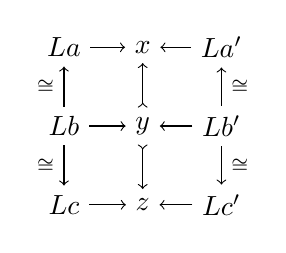
\begin{tikzpicture}
    \begin{scope}
        \node (1) at (0,2) {\( La \)};
        \node (2) at (1,2) {\( x \)};
        \node (3) at (2,2) {\( La' \)};
        \node (4) at (0,1) {\( Lb \)};
        \node (5) at (1,1) {\( y \)};
        \node (6) at (2,1) {\( Lb' \)};
        \node (7) at (0,0) {\( Lc \)};
        \node (8) at (1,0) {\( z \)};
        \node (9) at (2,0) {\( Lc' \)};
        \draw [->] (1) to node []
          {\scriptsize{\( \)}} (2);
        \draw [->] (3) to node []
          {\scriptsize{\( \)}} (2);
        \draw [->] (4) to node []
          {\scriptsize{\( \)}} (5);
        \draw [->] (6) to node []
          {\scriptsize{\( \)}} (5);
        \draw [->] (7) to node []
          {\scriptsize{\( \)}} (8);
        \draw [->] (9) to node []
          {\scriptsize{\( \)}} (8);
        \draw [->] (4) to node [left]
          {\scriptsize{\( \iso \)}} (1);
        \draw [->] (4) to node [left]
          {\scriptsize{\( \iso \)}} (7);
        \draw [>->] (5) to node []
          {\scriptsize{\( \)}} (2);
        \draw [>->] (5) to node []
          {\scriptsize{\( \)}} (8);
        \draw [->] (6) to node [right]
          {\scriptsize{\( \iso \)}} (3);
        \draw [->] (6) to node [right]
          {\scriptsize{\( \iso \)}} (9);
    \end{scope}
  \end{tikzpicture}
\]
%
As before, we associate to $ ( \StrCsp_L , P ) $ the new grammar
$ ( \StrCsp_L , P' ) $ where $ P' $ is the set of rules derived from
the rules in $ P $ using the double pushout approach.  In fact, this
association is functorial.  We then associate, again functorially, a
double category to $ ( \StrCsp_L , P' ) $ with objects from $ \A $,
vertical arrows are spans in $ \A $ with invertible legs, horizontal
arrows are structured cospans in $ \StrCsp_L $, and whose squares are
generated by the rules in $ P' $. The composite functor $ \Lang $ is
called the language functor.  As we see below, the language functor is
used to encode a rewriting relation on $ \X $ inside the double category
$ \Lang ( \StrCsp_L , P ) $.

Using a double cateogry allows us to combine into a single structure
the connectability (horizontal composition) and rewritability
(vertical composition) of structured cospans.  The fact that this
actually is a double category \cite[Lem.~4.2]{CicCour_SpCspTopos}
ensures the compatibility of connecting and rewriting via the
interchange law. This compatability grants us the ability to decompose
a system into subsystems, rewrite those, then connect the
results.

At this point, we begin to connect the rewriting relation on a grammar
$ ( \X , P ) $ with the language of a certain structured cospan
grammer $ ( \StrCsp_L , \hat{P} ) $.

One result Gadducci and Heckle rely on goes back to the expressiveness
of certain grammars given by Ehrig, et. al.~when they introdruced graph
rewriting.  That is, a set of rules
$ \{ \ell_j \monicgets k_j \monicto r_j \} $ has the same rewrite
relation as the set of rules
$ \{ \ell_j \monicgets k'_j \monicto r_j \} $ where $ k'_j $ is the
discrete graph underlying $ k_j $ \cite[Prop.~3.3]{Ehrig_GraphGram}.

Just as this fact was a keystone in Gadducci and Heckle's work, we
prove a modified version of it. To understand the following statement,
we use the notation $ P_\flat $ to refer to the set of rules obtained
from $ P = \{ \ell_j \monicgets k_j \monicto r_j \} $ by restricting
the the span lets along the counit $ LRk_j \to k_j $ of the comonad
$ LR $.

\begin{theorem*}[\ref{thm:production-same-rewrite-relation-as-discrete}]
Fix a geometric morphism $ L \dashv R \from \X \to \A $ with monic
counit. Let $ ( \X , P ) $ be a grammar such that for every
$ \X $-object $ x $ in the apex of a production of $ P $, the Heyting
algebra $ \Sub (x) $ is well-founded.  The rewriting relation for a
grammar $ ( \X , P ) $ is equal to rewriting relation for the grammar
$ ( \X , P_{\flat} ) $.
\end{theorem*}

It follows from this theorem that, instead of working with the
rewriting relation for $ ( \X , P ) $, we can instead study the
rewriting relation $ ( \X , P_\flat ) $ because it is the same.

Now, to decompose the systems in $ \X $ and the rules in $ P $, we
associate to $ ( \X , P ) $ the structured cospan grammar
$ ( \StrCsp_L , \hat{P} ) $ where $ \hat{P} $ contains
%
\[
  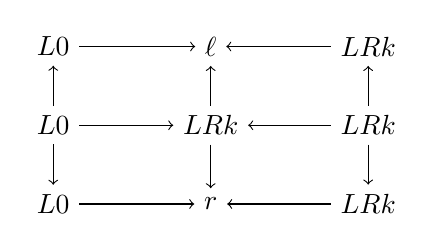
\begin{tikzpicture}
    \node (1) at (0,2) {$ L 0 $};
    \node (2) at (2,2) {$ \ell $};
    \node (3) at (4,2) {$ LRk $};
    \node (4) at (0,1) {$ L 0 $};
    \node (5) at (2,1) {$ LRk $};
    \node (6) at (4,1) {$ LRk $};
    \node (7) at (0,0) {$ L 0 $};
    \node (8) at (2,0) {$ r $};
    \node (9) at (4,0) {$ LRk $};
    \draw [->] (1) to node [] {\scriptsize{$  $}} (2);
    \draw [->] (3) to node [] {\scriptsize{$  $}} (2);
    \draw [->] (4) to node [] {\scriptsize{$  $}} (5);
    \draw [->] (6) to node [] {\scriptsize{$  $}} (5);
    \draw [->] (7) to node [] {\scriptsize{$  $}} (8);
    \draw [->] (9) to node [] {\scriptsize{$  $}} (8);
    \draw [->] (4) to node [] {\scriptsize{$  $}} (1);
    \draw [->] (4) to node [] {\scriptsize{$  $}} (7);
    \draw [->] (5) to node [] {\scriptsize{$  $}} (2);
    \draw [->] (5) to node [] {\scriptsize{$  $}} (8);
    \draw [->] (6) to node [] {\scriptsize{$  $}} (3);
    \draw [->] (6) to node [] {\scriptsize{$  $}} (9);
  \end{tikzpicture}
\]
% 
for every rule $ LRk \to \ell \times r $ of $ P_{\flat} $.

This structured cospan grammar effectively turns all of the systems $ x $
in $ \X $ into structured cospans $ L0 \to x \gets Lo $ without inputs
or outputs and turns the rules from $ P $ into what we can think of as
generaters $ \hat{P} $ for a double category.  The main result of the
paper is that the process complete encodes the rewriting relation for
$ ( \X,P ) $ inside of a vertical hom-set of a double category
generated by structured cospans.

\begin{theorem*}[\ref{thm:inductive-rewriting}]
  Fix a geometric morphism $ L \dashv R \from \X \to \A $ with monic
  counit. Let $ ( \X , P ) $ be a grammar such that for every
  $ \X $-object $ x $ in the apex of a production of $ P $, the
  Heyting algebra $ \Sub (x) $ is well-founded. Given $ g $,
  $ h \in \X $, then $ \deriv{g}{h} $ in the rewriting relation for a
  grammar $ ( \X , P ) $ if and only if there is a square
  %
  \[
    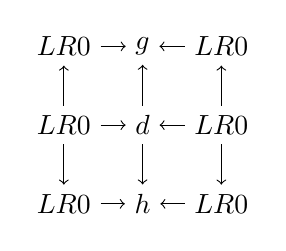
\begin{tikzpicture}
      \node (1t) at (0,2) {$ LR 0 $};
      \node (2t) at (1,2) {$ g $};
      \node (3t) at (2,2) {$ LR 0 $};
      \node (1m) at (0,1) {$ LR 0 $};
      \node (2m) at (1,1) {$ d $};
      \node (3m) at (2,1) {$ LR 0 $};
      \node (1b) at (0,0) {$ LR 0 $};
      \node (2b) at (1,0) {$ h $};
      \node (3b) at (2,0) {$ LR 0 $};
      \draw [->] (1t) to node [] {\scriptsize{$  $}} (2t);
      \draw [->] (3t) to node [] {\scriptsize{$  $}} (2t);
      \draw [->] (1m) to node [] {\scriptsize{$  $}} (2m);
      \draw [->] (3m) to node [] {\scriptsize{$  $}} (2m);
      \draw [->] (1b) to node [] {\scriptsize{$  $}} (2b);
      \draw [->] (3b) to node [] {\scriptsize{$  $}} (2b);
      \draw [->] (1m) to node [] {\scriptsize{$  $}} (1t);
      \draw [->] (1m) to node [] {\scriptsize{$  $}} (1b);
      \draw [->] (2m) to node [] {\scriptsize{$  $}} (2t);
      \draw [->] (2m) to node [] {\scriptsize{$  $}} (2b);
      \draw [->] (3m) to node [] {\scriptsize{$  $}} (3t);
      \draw [->] (3m) to node [] {\scriptsize{$  $}} (3b);
    \end{tikzpicture}
  \]
  % 
  in the double category $ \Lang ( \StrCsp_L , \hat{P} ) $.
\end{theorem*}

The hypothesis of this theorem are more mild than they seem.  Asking
for a monic counit is means that the comonad for this adjunction is
restricting a system, that is object of $ \X $, to the subobject
consisting of all the system components that can serve as an
interface.  Asking that the subobject algebra be well-founded is not
too restrictive given that systems of interest are typically finite
anyway.

Because this theorem completely characterizes the rewriting relation
as squares framed by $ 0 $ inside of a double category, given any
decomposition of a system $ x $ into structured cospans
%
\[
  L0 \to x_1 \gets La_1 \to x_2 \gets La_2 \dotsm La_{n-1} \to x_n
  \gets L0
\]
%
we can rewrite each of these structured cospans independently using
rewriting rules on these subsystems. This will give a pasting diagram
of the sort
%
\[
  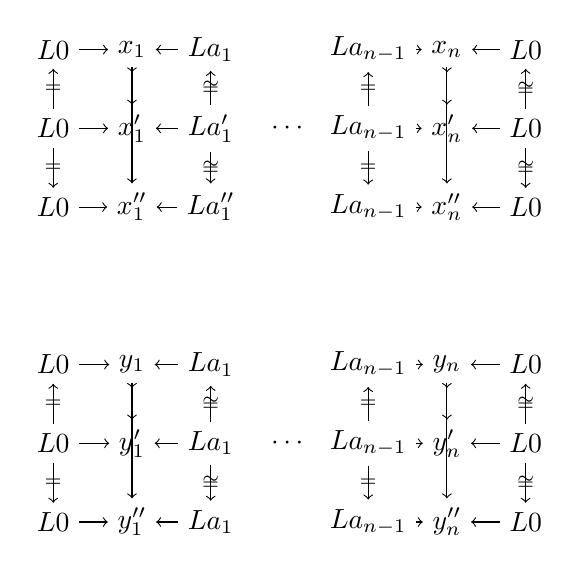
\begin{tikzpicture}
    \begin{scope}[shift={(0,4)}]
      \node (1) at (0,2) {$ L0 $};
      \node (2) at (1,2) {$ x_1 $};
      \node (3) at (2,2) {$ La_1 $};
      \node (4) at (0,1) {$ L0 $};
      \node (5) at (1,1) {$ x'_1 $};
      \node (6) at (2,1) {$ La'_1 $};
      \node (7) at (0,0) {$ L0 $};
      \node (8) at (1,0) {$ x''_1 $};
      \node (9) at (2,0) {$ La''_1 $};
      \draw [->] (1) to node [] {\scriptsize{$  $}} (2);
      \draw [->] (3) to node [] {\scriptsize{$  $}} (2);
      \draw [->] (4) to node [] {\scriptsize{$  $}} (5);
      \draw [->] (6) to node [] {\scriptsize{$  $}} (5);
      \draw [->] (7) to node [] {\scriptsize{$  $}} (8);
      \draw [->] (9) to node [] {\scriptsize{$  $}} (8);
      \draw [->] (4) to node [] {\scriptsize{$ = $}} (1);
      \draw [->] (4) to node [] {\scriptsize{$ = $}} (7);
      \draw [>->] (2) to node [] {\scriptsize{$  $}} (5);
      \draw [->] (2) to node [] {\scriptsize{$  $}} (8);
      \draw [->] (6) to node [] {\scriptsize{$ \cong  $}} (3);
      \draw [->] (6) to node [] {\scriptsize{$ \cong $}} (9);
    \end{scope}
    %
    \begin{scope}[shift={(4,4)}]
      \node (1) at (0,2) {$ La_{n-1} $};
      \node (2) at (1,2) {$ x_n $};
      \node (3) at (2,2) {$ L0 $};
      \node (4) at (0,1) {$ La_{n-1} $};
      \node (5) at (1,1) {$ x'_n $};
      \node (6) at (2,1) {$ L0 $};
      \node (7) at (0,0) {$ La_{n-1} $};
      \node (8) at (1,0) {$ x''_n $};
      \node (9) at (2,0) {$ L0 $};
       \draw [->] (1) to node [] {\scriptsize{$  $}} (2);
      \draw [->] (3) to node [] {\scriptsize{$  $}} (2);
      \draw [->] (4) to node [] {\scriptsize{$  $}} (5);
      \draw [->] (6) to node [] {\scriptsize{$  $}} (5);
      \draw [->] (7) to node [] {\scriptsize{$  $}} (8);
      \draw [->] (9) to node [] {\scriptsize{$  $}} (8);
      \draw [->] (4) to node [] {\scriptsize{$ = $}} (1);
      \draw [->] (4) to node [] {\scriptsize{$ = $}} (7);
      \draw [>->] (2) to node [] {\scriptsize{$  $}} (5);
      \draw [->] (2) to node [] {\scriptsize{$  $}} (8);
      \draw [->] (6) to node [] {\scriptsize{$ \cong  $}} (3);
      \draw [->] (6) to node [] {\scriptsize{$ \cong $}} (9);
    \end{scope}
    %
    \begin{scope}
      \node (1) at (0,2) {$ L0 $};
      \node (2) at (1,2) {$ y_1 $};
      \node (3) at (2,2) {$ La_1 $};
      \node (4) at (0,1) {$ L0 $};
      \node (5) at (1,1) {$ y'_1 $};
      \node (6) at (2,1) {$ La_1 $};
      \node (7) at (0,0) {$ L0 $};
      \node (8) at (1,0) {$ y''_1 $};
      \node (9) at (2,0) {$ La_1 $};
       \draw [->] (1) to node [] {\scriptsize{$  $}} (2);
      \draw [->] (3) to node [] {\scriptsize{$  $}} (2);
      \draw [->] (4) to node [] {\scriptsize{$  $}} (5);
      \draw [->] (6) to node [] {\scriptsize{$  $}} (5);
      \draw [->] (7) to node [] {\scriptsize{$  $}} (8);
      \draw [->] (9) to node [] {\scriptsize{$  $}} (8);
      \draw [->] (4) to node [] {\scriptsize{$ = $}} (1);
      \draw [->] (4) to node [] {\scriptsize{$ = $}} (7);
      \draw [>->] (2) to node [] {\scriptsize{$  $}} (5);
      \draw [->] (2) to node [] {\scriptsize{$  $}} (8);
      \draw [->] (6) to node [] {\scriptsize{$ \cong  $}} (3);
      \draw [->] (6) to node [] {\scriptsize{$ \cong $}} (9);
    \end{scope}
    %
    \begin{scope}[shift={(4,0)}]
      \node (1) at (0,2) {$ La_{n-1} $};
      \node (2) at (1,2) {$ y_n $};
      \node (3) at (2,2) {$ L0 $};
      \node (4) at (0,1) {$ La_{n-1} $};
      \node (5) at (1,1) {$ y'_n $};
      \node (6) at (2,1) {$ L0 $};
      \node (7) at (0,0) {$ La_{n-1} $};
      \node (8) at (1,0) {$y''_n $};
      \node (9) at (2,0) {$ L0 $};
       \draw [->] (1) to node [] {\scriptsize{$  $}} (2);
      \draw [->] (3) to node [] {\scriptsize{$  $}} (2);
      \draw [->] (4) to node [] {\scriptsize{$  $}} (5);
      \draw [->] (6) to node [] {\scriptsize{$  $}} (5);
      \draw [->] (7) to node [] {\scriptsize{$  $}} (8);
      \draw [->] (9) to node [] {\scriptsize{$  $}} (8);
      \draw [->] (4) to node [] {\scriptsize{$ = $}} (1);
      \draw [->] (4) to node [] {\scriptsize{$ = $}} (7);
      \draw [>->] (2) to node [] {\scriptsize{$  $}} (5);
      \draw [->] (2) to node [] {\scriptsize{$  $}} (8);
      \draw [->] (6) to node [] {\scriptsize{$ \cong  $}} (3);
      \draw [->] (6) to node [] {\scriptsize{$ \cong $}} (9);
    \end{scope}
    %
    \node () at (3,5) {$ \dotsm $};
    \node () at (1,3) {$ \dotsv $};
    \node () at (3,1) {$ \dotsm $};
    \node () at (5,3) {$ \dotsv $};
  \end{tikzpicture}
\]
%
Then we can compose these squares in any order to get a rewriting on
the original system $ x $ as desired.

The structure of this paper is as follows.  Section \ref{sec:StrCsp}






% ~~~~~~~~~~~~~~~~~~~~~~~~~~~~~~~~~~~~~~~~
% 
% ~~~~~~~~~~~ bibliography ~~~~~~~~~~~~~~~
% 
% ~~~~~~~~~~~~~~~~~~~~~~~~~~~~~~~~~~~~~~~~

\begin{thebibliography}{99}
  % use APA style
  % \bibitem{1st-citation}

\bibitem{StrCsp} J.~Baez, K.~Courser. Structured cospans. \emph{In preparation}.

\bibitem{NetMods} J.~Baez, J.~Foley, J.~Moeller, B.~Pollard. Network
  Models. \emph{arXiv preprint} arXiv:1711.00037. 2017.
  
\bibitem{PassiveNets} J.~Baez, B.~Fong. A compositional framework for passive linear networks. \emph{arXiv preprint} arXiv:1504.05625. 2015.

\bibitem{MrkvProc} J.~Baez, B.~Fong, B.~Pollard. A compositional
  framework for Markov processes. \emph{J.~Math.~Phys.} 57, No.~3:
  033301. 2016.
  
\bibitem{RxNets} J.~Baez, B.~Pollard. A compositional framework for
  reaction networks. \emph{Rev. Math. Phys.} 29, No.~9, 1750028. 2017.

\bibitem{OpenPetri} J.~Baez, J.~Master. Open Petri Nets. \emph{arXiv preprint} arXiv:1808.05415. 2018.
  
\bibitem{Chomsky} N.~Chomsky. On Certain Formal Properties of Grammars.
\emph{Inf.~Control}. No.~2. 137-167. 1959. 
  
\bibitem{Cic_SpCsp} D.\ Cicala. Spans of cospans. \emph{Theory Appl.\
    Categ.} 33, No.\ 6, 131--147. 2018.

\bibitem{CicCour_SpCspTopos} D.\ Cicala and K.\ Courser. Spans of
  cospans in a topos. \emph{Theory Appl.\ Categ.} 33, No.\ 1,
  1--22. 2018.

\bibitem{DixKiss_OpenGraphs} L.\ Dixon, and A.\ Kissinger. Open-graphs
  and monoidal theories. \emph{Math.\ Structures Comput.\ Sci.},
  \textbf{23}, No.\ 2, 308--359. 2013.

\bibitem{Ehrig_GraphGram} H.\ Ehrig, M.\ Pfender, and H.J.\
  Schneider. Graph-grammars: An algebraic approach. In \emph{Switching
    and Automata Theory, 1973. SWAT'08. IEEE Conference Record of 14th
    Annual Symposium on}, 167--180. IEEE. 1973.
  
\bibitem{DecorCsp} B.\ Fong. Decorated cospans. \emph{Theory
    Appl.\ Categ.} 30, Paper No.\ 33, 1096--1120. 2015.
          
\bibitem{Gadd_IndGraphTrans} F.\ Gadducci, R.\ Heckel. An inductive
  view of graph transformation.\emph{International Workshop on
    Algebraic Development Techniques}. 223--237. Springer, Berlin. 1998.

\bibitem{DblPushoutRevis} A.~Habel, J.~M\:{u}ller,
  D.~Plump. Double-pushout graph transformation
  revisited. \emph{Math. Structures Comput. Sci.}
  11. No.~5. 637--688. 2001).
  
\bibitem{LackSobo_Adhesive} S.\ Lack, and P.\ Soboci\'{n}ski. Adhesive
  categories. In \emph{International Conference on Foundations of
    Software Science and Computation Structures}, 273--288. Springer,
  Berlin, Heidelberg. 2004.

\bibitem{LackSobo_ToposIsAdh} S.~Lack, P.~Soboci\'{n}ski. Toposes are adhesive. \emph{International Conference on Graph Transformation}. Springer, Berlin, Heidelberg. 2006.

\bibitem{ShulDblCat} M.~Shulman. Constructing symmetric monoidal bicategories. \emph{arXiv preprint} arXiv:1004.0993. 2010.
  
\bibitem{Wraith_ArtinGlue} G.\ Wraith. Artin gluing. \emph{J.\ Pure
    Appl.\ Algebra} \textbf{4}, 345--348. 1974.

\end{thebibliography}
\end{document}
